\documentclass{scrartcl}

\usepackage[a4paper,hmargin={2.54cm,2.54cm},vmargin={3.17cm,3.17cm}]{geometry}
\usepackage{sectsty}
\allsectionsfont{\rmfamily\textbf}

\usepackage{amsmath,amssymb,amsthm,amstext,booktabs,subfig,epstopdf,graphicx,tabularx,algorithm}
\usepackage{algpseudocode,algorithmicx}
\usepackage{enumerate}

\usepackage{natbib}

\def\Or{\textrm{ or }}
\def\And{\textrm{ and }}
\newcommand{\med}[1]{\mathrm{med}\left(#1\right)}
%\def\mod{\textrm{ mod }}
\renewcommand{\Pr}[1]{\mathbf{Pr}\left[#1\right]}
\newcommand{\E}[1]{\mathbb{E}\left[#1\right]}
\newcommand{\Var}[1]{\mathrm{Var}\left[#1\right]}

%head and foot
\usepackage{fancyhdr}
\pagestyle{fancy}
\lhead{COSC-548: \emph{Streaming Algorithms}}
\chead{Final Project Report}
\rhead{Shuo Liu}
\lfoot{}
\cfoot{\thepage}
\rfoot{}
%\numberwithin{equation}{chapter}
\usepackage[runin]{abstract}

\usepackage[pdfborder={0 0 0},colorlinks=true,citecolor=blue,linkcolor=blue,CJKbookmarks=true]{hyperref}

\setlength{\absleftindent}{1.5cm} \setlength{\absrightindent}{1.5cm}
\setlength{\abstitleskip}{-\parindent}
\setlength{\absparindent}{0cm}

\newtheorem{definition}{Definition}
\newtheorem{theorem}{Theorem}
\newtheorem{remark}{Remark}
\newtheorem{problem}{Problem}

\renewcommand{\algorithmicrequire}{\textbf{Input:}} % Use Input in the format of Algorithm
\renewcommand{\algorithmicensure}{\textbf{Output:}} % Use Output in the format of Algorithm

\bibliographystyle{unsrtnat}

\makeatletter
\DeclareOldFontCommand{\rm}{\normalfont\rmfamily}{\mathrm}
\DeclareOldFontCommand{\sf}{\normalfont\sffamily}{\mathsf}
\DeclareOldFontCommand{\tt}{\normalfont\ttfamily}{\mathtt}
\DeclareOldFontCommand{\bf}{\normalfont\bfseries}{\mathbf}
\DeclareOldFontCommand{\it}{\normalfont\itshape}{\mathit}
\DeclareOldFontCommand{\sl}{\normalfont\slshape}{\@nomath\sl}
\DeclareOldFontCommand{\sc}{\normalfont\scshape}{\@nomath\sc}
\makeatother

%%%%%%%%%%%%%%%%%%%导言区设置完毕
%%%%%%%%%%%%%%%%%%%%%%%%%%%%%%%%%%%%%%%%%%%%%%%%%%%%%%%%%%%%%%%%%%%%%
\begin{document}
\pagestyle{plain}
%Header-Make sure you update this information!!!!
\noindent
\large\textbf{Final Project Report} \hfill \textbf{Shuo Liu} \\
\normalsize COSC-548: \emph{Streaming Algorithms} \hfill \today 
\vspace{-5pt}
\noindent\rule{\textwidth}{0.5pt}

\section{Introduction}

\subsection{Theory part} % (fold)
\label{sub:theory_part}

This is a report on empirical experiments of a streaming algorithm proposed in the paper \citep{chakrabarti2010near}. The algorithm gives an $(\varepsilon,\delta)$-approximation of its empirical entropy of a given stream. 

\begin{definition}
For a data stream $A=\langle a_1, a_2,...,a_m\rangle$, with each \emph{token} $a_j\in[n]$, the \emph{empirical probability distribution} of the stream is $p=(p_1,p_2,...,p_n)$, where $p_i=m_i/m$ and $m_i=\{j:a_j=i\}$, $\forall i\in[n]$. The \emph{empirical entropy} of $A$ is $H(p)=\sum_{i=1}^n-p_i\log_2{p_i}$.
\end{definition}

Notice that the definition of the empirical entropy makes it an average on a real-valued function $f$ such that $f(0)=0$:
$$\overline{f}(A;m)=\frac{1}{m}\sum_{i=1}^nf(m_i),$$
where our $f(m_i)=m_i\log(m/m_i)$. \citet{Alon:1996:SCA:237814.237823} proposed a method to estimate quantities of this form $\overline{f}(A;m)$, and the paper \citep{chakrabarti2010near} bases the algorithm on this research.

Let $\mathcal{D}(A)$ be the distribution of the random variable $R$ defined thus: Pick $J\in[m]$ uniformly at random and $R=|\{j:a_j=a_J, J\leq j\leq m\}|$. By choosing a positive integer $c$, the value of $\textrm{Est}_f(R,c)=\frac{1}{c}\sum_{i=1}^cX_i$ can be arbitrarily close to $\overline{f}(A;m)$, where $\{X_i\}$ are independent and identically distributed to $(f(R)-f(R-1))$. Therefore, by selecting $c$ properly, we can calculate a $(\varepsilon, \delta)$-approximation of the empirical entropy of a stream.

Define a function $\lambda_m(x)=x\log_2(m/x)$, where $\lambda_m(0)=0$. Clearly, $\overline{\lambda}_m(A;m)=H(p)$. By defining $X=\lambda_m(R)-\lambda_m(R-1)$, it can be proved that: if $p_{\max}=\max_ip_i$ is bounded far from 1, then $1/\E{X}$ is ``small'' and $\textrm{Est}_{\lambda_m}(R,c)$ gives a good estimator with a ``small'' value of $c$; while if $p_{\max}>\frac{1}{2}$, corresponding $R'$ of the stream $A'$ which is the stream $A$ removing the most frequent token can be recovered and $1/\E{X'}$ is also ``small'', so that $\textrm{Est}_{\lambda_m}(R',c)$ along with the estimation of $p_{\max}$ becomes a good estimator of $H(p)$.

Noticed that the algorithm as described above also requires an estimation of $p_{\max}$. The task can be done by maintain a frequency estimator of tokens in parallel. One algorithm proposed (and also used in the implementation) is Misra-Gries algorithm \citep{Misra:1982:FRE:867576}. The estimation $\hat{m}_i$ on token $i\in[n]$ satisfies $0\leq m_i-\hat{m}_i\leq(m-m_i)/k$ (\citep{Bose2003BoundsFF}).

The paper \citep{chakrabarti2010near} proves that

\begin{theorem}
The proposed algorithm uses $O(\varepsilon^{-2}\log{(\delta^{-1})\log{m(\log{m}+\log{n})}})$ bits of space and gives an $(\varepsilon, \delta)$-approximation to $H(p)$.
\end{theorem}
\begin{theorem}
The proposed algorithm can be implemented such that a length $m$ stream can be processed in $O((m+\log^3{m}\varepsilon^{-2}\log{(\delta^{-1})})(\log{\varepsilon^{-1}+\log\log{\delta^{-1}}+\log\log{m}}))$.
\label{thm2}
\end{theorem}
% subsection theory_part (end)

\subsection{Implementation part} % (fold)
\label{sub:implementation_part}

The authors proposed 2 implementations. The first one (\emph{original}) directly implements the idea that we keep tracking $R$ and $R'$ as defined in Section \ref{sub:theory_part} above. The second one (\emph{fast}) implements with pre-calculation of when should we change the sample we are keeping, by adapting the idea of reservoir sampling \citep{Vitter:1985:RSR:3147.3165}, and store these calculations with heaps. Note that by using heaps, the asymptotic space cost remains unchanged, since the space usage of each estimator only multiplies by a constant number.

Also note that in both algorithms the paper described that the random integer generators utilize the size of the stream $m$, therefore it is necessary for the algorithm to know the size of the stream before the stream begins, which is impossible in applications. However, it is actually possible to run the algorithms without $m$, because since in calculations, the random numbers are always divided by the same number ($m^3$), we can replace such integer generators with float number generators in range of [0,1], that is we are directly generating numbers after their division by $m^3$.
% subsection implementation_part (end)

\section{Experiments} % (fold)
\label{sec:experiments}
\subsection{Environment and settings} % (fold)
\label{sub:environment}
The two algorithms (original and fast) are implemented using Java 8. Tests are run on a computer with Intel(R) Core(TM) i7-7700HQ CPU @ 2.80GHz and 15.8GB RAM. Random number generators are those under the package \texttt{java.util}. Heaps are self-implemented. Several Java \texttt{Collection} classes are used. The results regarding running time are only for comparison between this two methods.

The streams for experiments are randomly generated and follows power distributions: 
\begin{equation*}
	f(x;\lambda)=\begin{cases}
		\lambda e^{-\lambda x}, & x\geq0, \\
		0, & x<0,
	\end{cases}
\end{equation*}
with different $\lambda$'s ($\lambda>0$), so that the frequencies of some few tokens would be significantly higher than the others. On the other hand, when $\lambda$ is smaller, the variance of frequencies of tokens drops.
% subsection environment (end)

\subsection{Results} % (fold)
\label{sub:results}
The results of the experiments are discussed in this section.

Data streams are generated in different sizes. Then the two algorithms are run multiple times with different random seeds, and the results are averaged. The accurate empirical entropy are also calculated for each data stream for comparison. In order to check multiplicative errors, those runs with results out of the multiplicative range are marked out. The definition of $(\varepsilon,\delta)$-multiplicative error is
\begin{equation}
	\Pr{|\mathcal{A}(\sigma)-\Phi{\sigma}|>\varepsilon\cdot\Phi(\sigma)}\leq1-\delta,
	\label{eq}
\end{equation}
where $\mathcal{A}(\sigma)$ and $\Phi(\sigma)$ are the result of an algorithm and the accurate answer over a stream $\sigma$ respectively.

The algorithms are tested on datasets of different sizes and in different distributions. How parameters changes are shown in Table \ref{tb:1}, where $m$ is the size of the stream and $n$ is the domain size.

\begin{table}[htbp]
\centering
\begin{tabularx}{.98\textwidth}{c|llll|c}
\toprule
\# &\multicolumn{4}{c}{Fixed parameters} & Independent variable \\
\midrule
1&$m=10^5$ & $n=10000$ & $\varepsilon=0.1$ & $\delta=0.4$ & $\lambda(=0.02,0.1,0.2,0.4,1.0,2.0)$\\
2&$\lambda=1.0$ & $n=1000$ & $\varepsilon=0.1$ & $\delta=0.2$ & $m(=5\times10^3,10^4,5\times10^4,10^5,5\times10^5,10^6)$\\
3&$\lambda=1.0$ & $m=10^5$ & $\varepsilon=0.5$ & $\delta=0.4$ & $n(=1000,2000,5000,10000)$\\
4&$m=10^5$ & $n=1000$ & $\lambda=0.4$ & $\delta=0.2$ & $\varepsilon(=0.1,0.2,0.5,0.8)$\\
5&$m=10^5$ & $n=1000$ & $\lambda=1.0$ & $\varepsilon=0.5$ & $\delta(=0.2,0.4,0.6,0.8)$\\
\bottomrule
\end{tabularx}
\caption{Parameter settings}
\label{tb:1}
\end{table}

In all experiments, the average results of 20 runs are very close to the corresponding accurate entropies, and the failure rate (\emph{i.e.} the chances that a result is out of the range defined by (\ref{eq})) are always 0. The paper proved that of the both algorithms the failure rate is lower than $\delta$; experiments show this is not a close bound. Detailed running results are shown in the appendix in Table \ref{tb:2}.

However, standard error of some experiments might change when their independent variable changes. Standard error shows how close the result of algorithms would be to the accurate one. Shown in Figure \ref{fig1}, (a) standard error drops when $\lambda$ increases, or the data stream is ``long-tailed''. If the frequencies of tokens are close (also entropy is high), the standard error of both algorithms would be high; (b)(c) standard error raises when $\epsilon$ and $\delta$ increase, which is natural as the algorithms would become inaccurate because the number of samplers $c$drops. On the other hand, standard error would not change with the size of data stream, or the domain size.

The experiments also show that the \emph{fast} algorithm runs significantly faster than the \emph{original} algorithm. Shown in Figure \ref{fig2}, the average running times of the fast algorithm are 50 to 100 times smaller than the original one's. Notice that Figure \ref{fig2b} indicates the running time increases linearly as the stream size increases, which has also been stated in the Theorem \ref{thm2} that $m$ dominates the running time of the algorithm. Figures \ref{fig2d} and \ref{fig2e} also show the relationship between running time and $\varepsilon$ or $\delta$ (quadratic and log-linear).

\begin{figure}[pt]
\centering
\subfloat[]{
	\begin{minipage}[t]{0.33\linewidth}
	\centering
	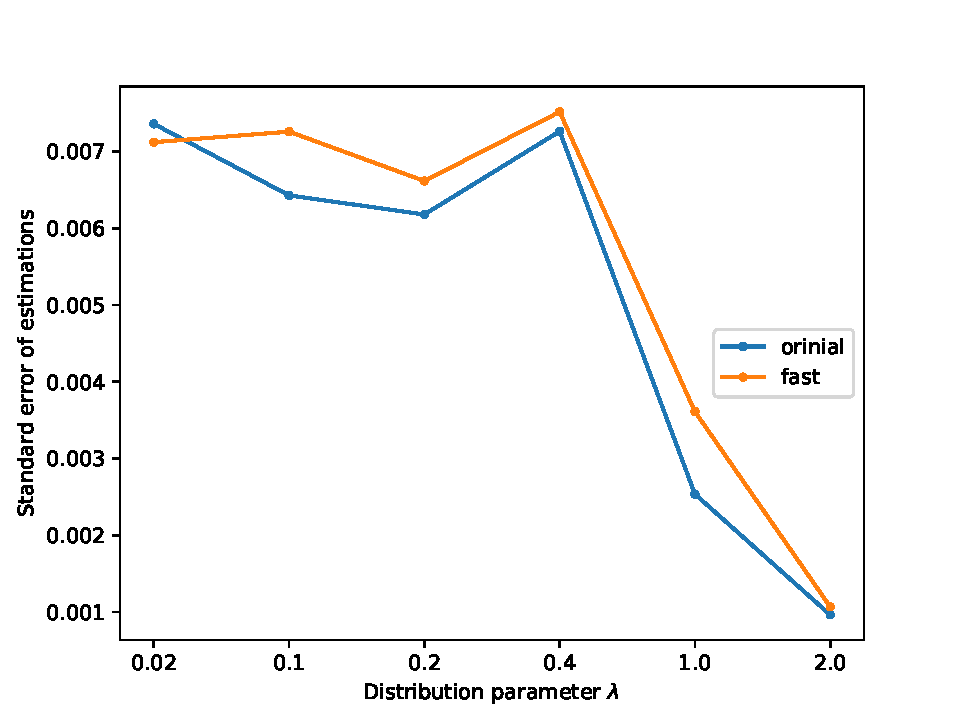
\includegraphics[width=2.2in]{Figure_lambda.pdf}
	\end{minipage}
}
\subfloat[]{
	\begin{minipage}[t]{0.33\linewidth}
	\centering
	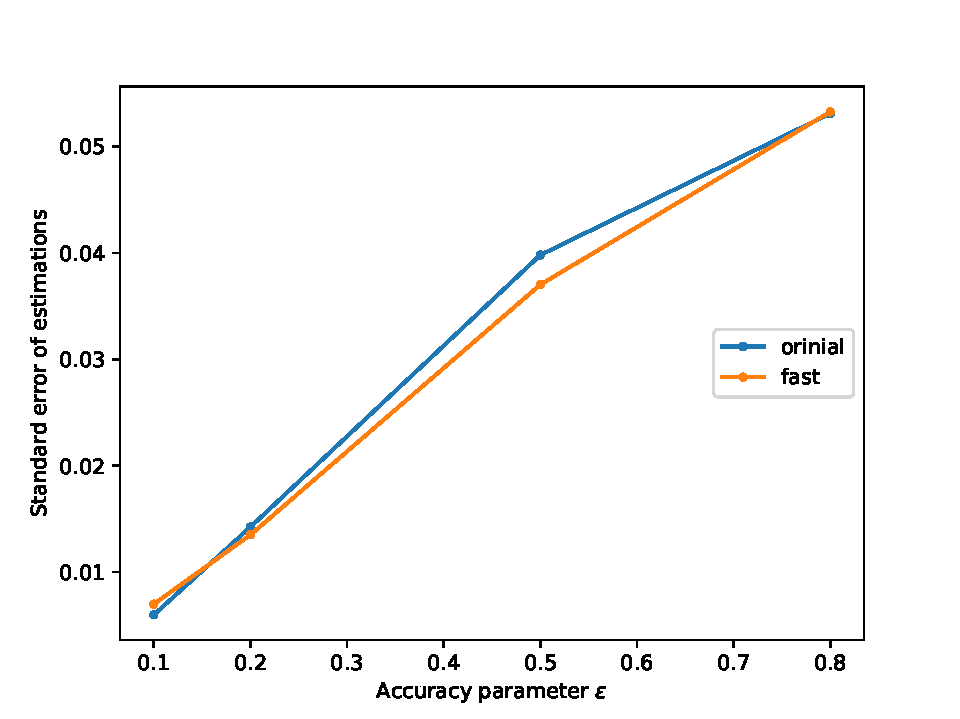
\includegraphics[width=2.2in]{Figure_epsilon.pdf}
	\end{minipage}
}
\subfloat[]{
	\begin{minipage}[t]{0.33\linewidth}
	\centering
	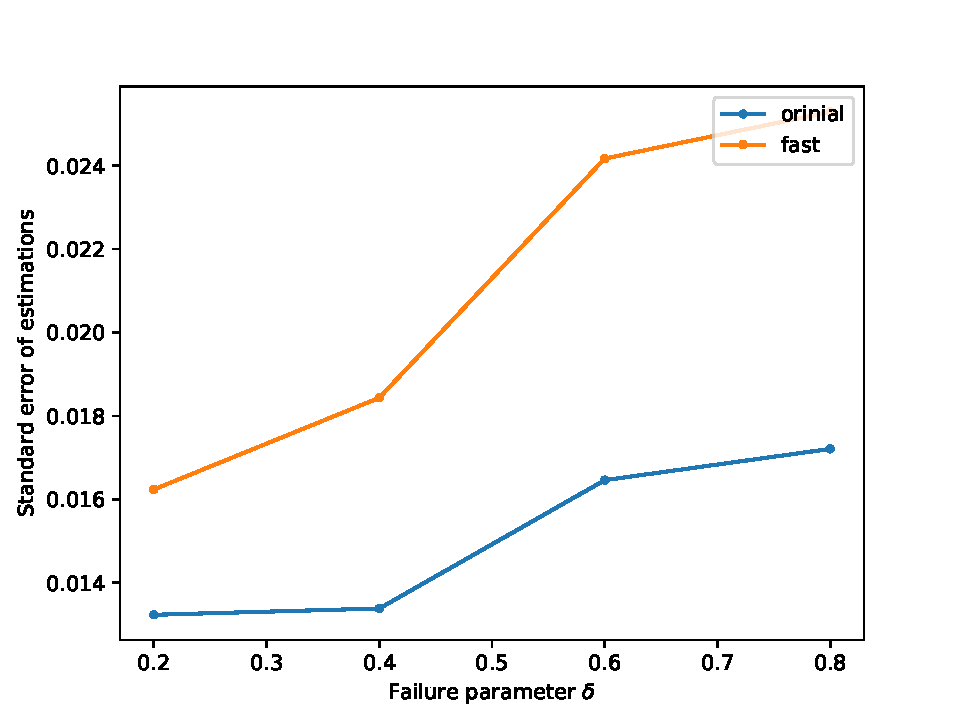
\includegraphics[width=2.2in]{Figure_delta.pdf}
	\end{minipage}
}
\caption{These three figures show how the standard error of results changes with (a) the distribution parameter $\lambda$, (b) the accuracy parameter $\epsilon$, and (c) the failure parameter $\delta$.}
\label{fig1}
\end{figure}

\begin{figure}[t]
\centering
\subfloat[]{
	\begin{minipage}[t]{0.33\linewidth}
	\centering
	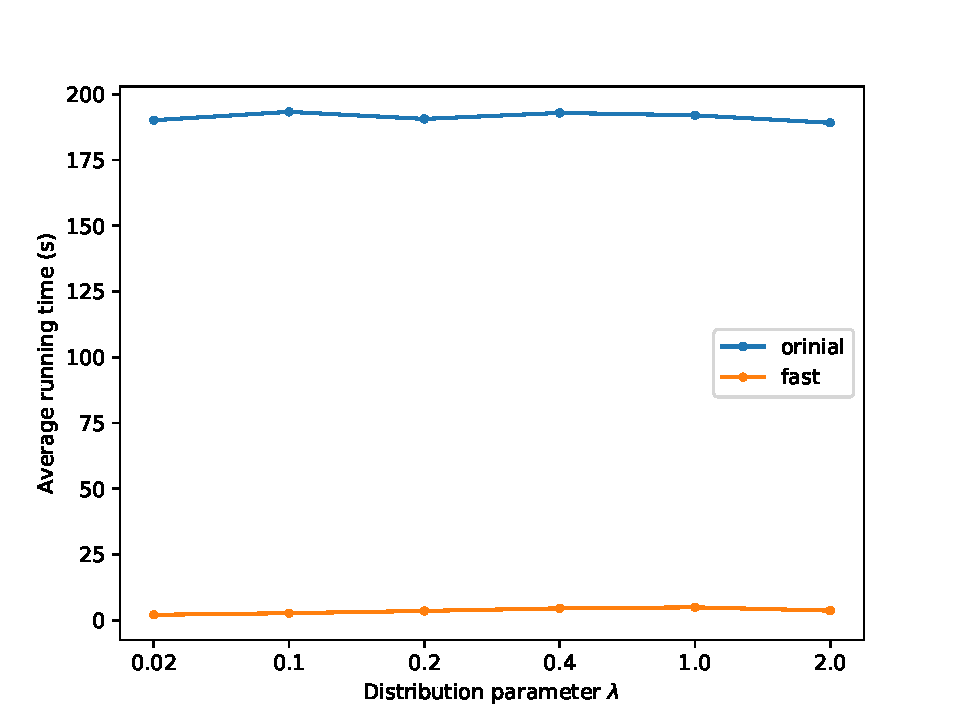
\includegraphics[width=2.2in]{Figure_lambda_time.pdf}
	\end{minipage}
}
\subfloat[]{
	\label{fig2b}
	\begin{minipage}[t]{0.33\linewidth}
	\centering
	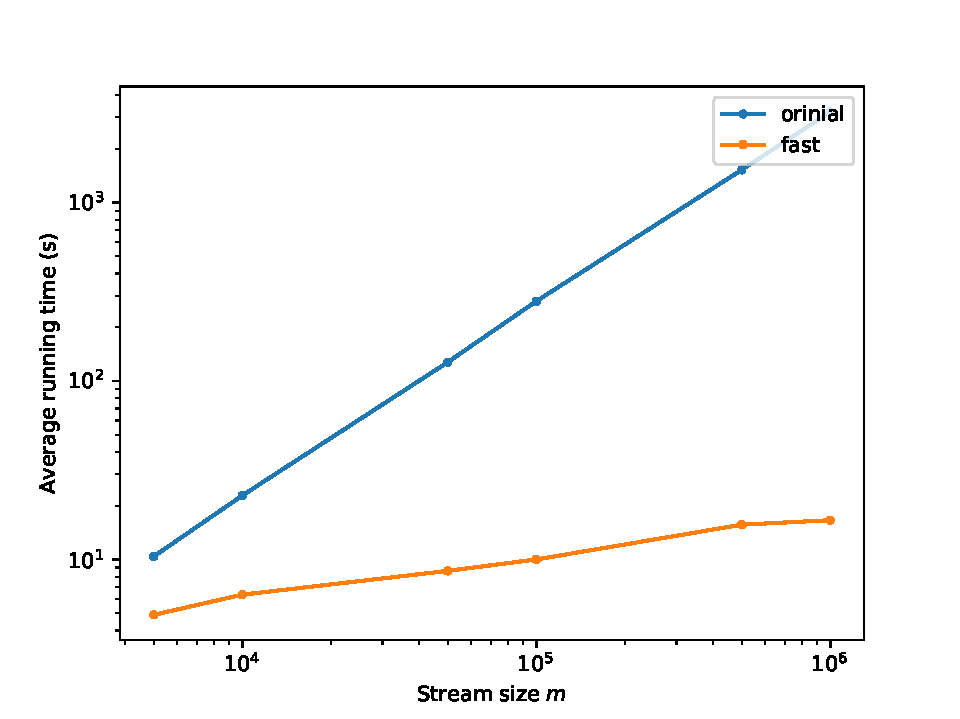
\includegraphics[width=2.2in]{Figure_m_time.pdf}
	\end{minipage}
}
\subfloat[]{
	\begin{minipage}[t]{0.33\linewidth}
	\centering
	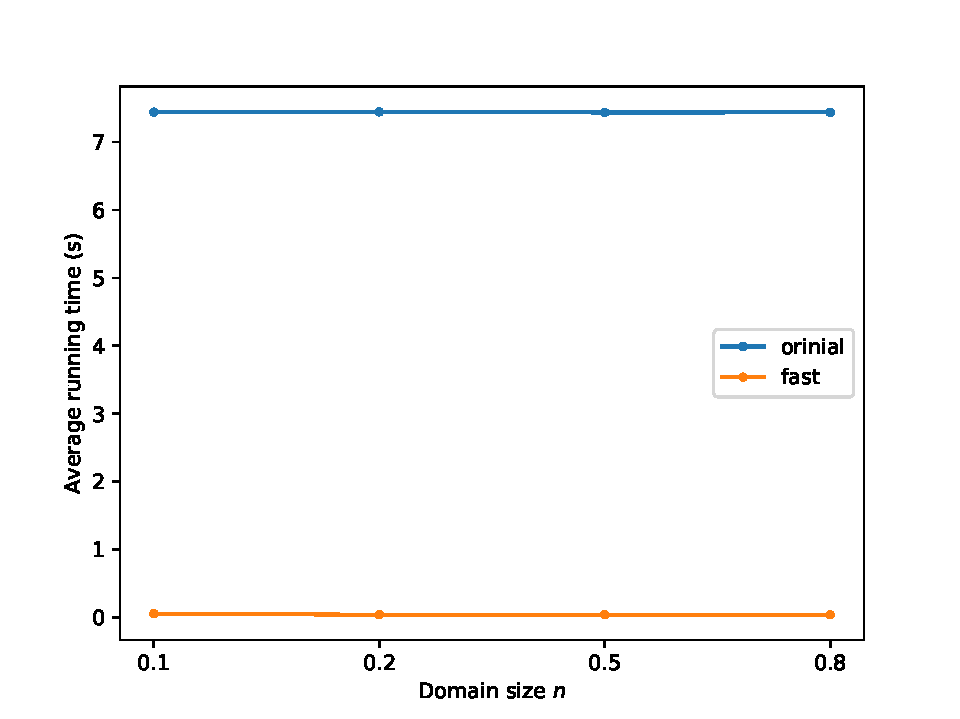
\includegraphics[width=2.2in]{Figure_n_time.pdf}
	\end{minipage}
}

\subfloat[]{
	\label{fig2d}
	\begin{minipage}[t]{0.33\linewidth}
	\centering
	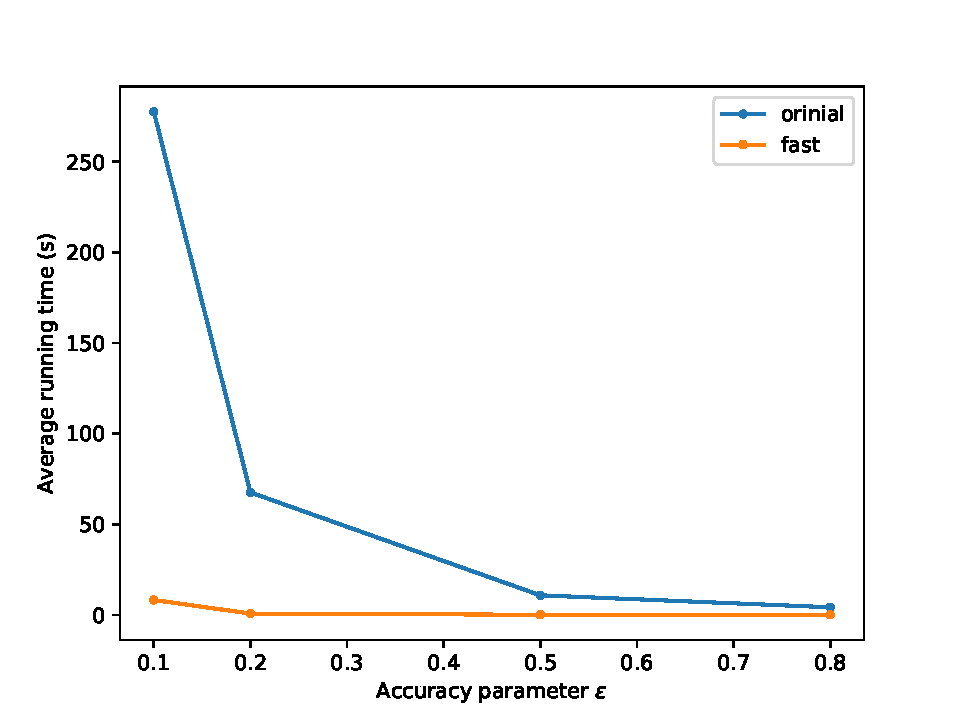
\includegraphics[width=2.2in]{Figure_epsilon_time.pdf}
	\end{minipage}
}
\subfloat[]{
	\label{fig2e}
	\begin{minipage}[t]{0.33\linewidth}
	\centering
	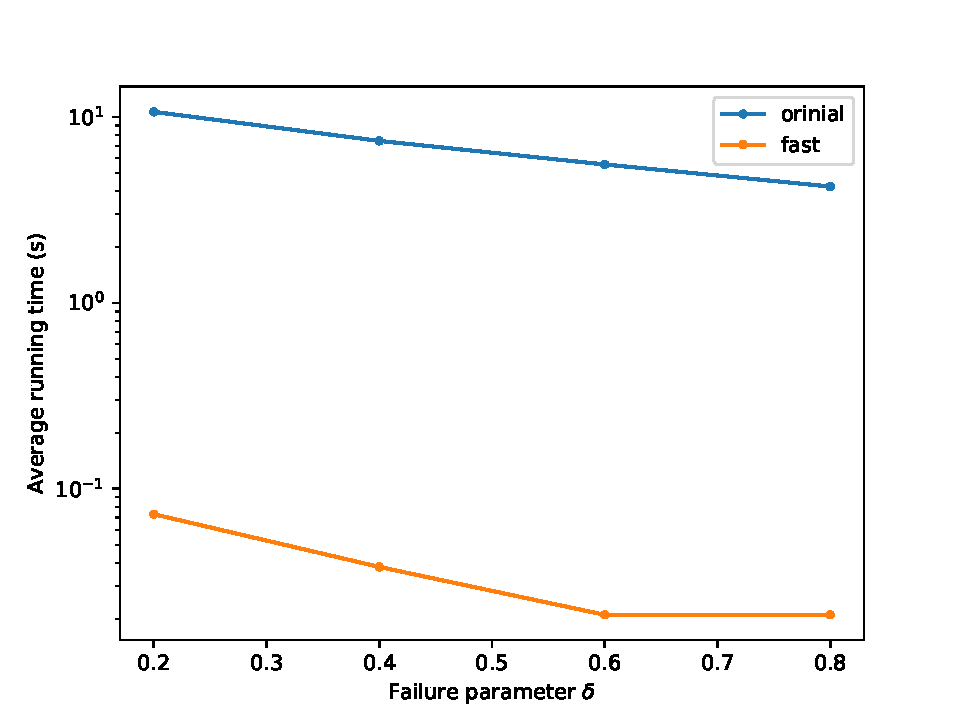
\includegraphics[width=2.2in]{Figure_delta_time.pdf}
	\end{minipage}
}
\caption{These five figures show how the standard error of results changes with (a) the distribution parameter $\lambda$, (b) the dataset size $m$, and the domain size $n$ in the first row; and (d) the accuracy parameter $\epsilon$, and (e) the failure parameter $\delta$ in the second row.}
\label{fig2}
\end{figure}
% subsection results (end)
% section experiments (end)

\section{Conclusion} % (fold)
\label{sec:conclusion}
The algorithm proposed in the paper \citep{chakrabarti2010near} could effectively estimate the empirical entropy of a given stream with multiplicative error $(\varepsilon,\delta)$, given the size of the size of tokens $n$. The \emph{fast} version of the algorithm significantly improves the efficiency of estimation. 

One way to improve the performance of this algorithm is to use a better frequency estimator rather than Misra-Grise. This can be a future work.
% section conclusion (end)
\bibliography{bibliography}

\subsection*{Appendix} % (fold)
\label{sub:appendix}
Detailed running results are shown below in Table \ref{tb:2}.
\begin{table}[h]
\centering
\begin{tabularx}{\textwidth}{c|c|c|c|ccc|ccc}
\toprule
\# & Ind. Var. & $m_{\max} $ & Accurate & \multicolumn{3}{c}{\emph{orinial}} & \multicolumn{3}{c}{\emph{fast}} \\
 &  &  &  & ave. & stderr & rtime(s) & ave. & stderr & rtime(s) \\
\midrule
1($\lambda$) & 0.02 & 685 & 7.08 & 7.08& 7.36E-03 & 190 & 7.08 & 7.12E-03 & 2.0 \\
 & 0.1 & 9424 & 4.77 & 4.77 & 6.43E-03 & 193 & 4.76 & 7.25E-03 & 2.6 \\
 & 0.2 & 18068 & 3.76 & 3.76 & 6.17E-03 & 190 & 3.76 & 6.61E-03 & 3.5 \\
 & 0.4 & 32954 & 2.77 & 2.77 & 7.26E-03 & 192 & 2.77 & 7.51E-03 & 4.5 \\
 & 1 & 63382 & 1.50 & 1.50 & 2.53E-03 & 191 & 1.52 & 3.61E-03 & 4.9 \\
 & 2 & 86315 & 0.66 & 0.66 & 9.64E-04 & 189 & 0.69 & 1.06E-03 & 3.6 \\
\midrule
2($m$) & 5000 & 3111 & 1.52 & 1.52 & 2.10E-03 & 10 & 1.54 & 2.60E-03 & 4.89\\
 & 10000 & 6253 & 1.51 & 1.51 & 1.98E-03 & 23 & 1.53 & 2.56E-03 & 6.34\\
 & 50000 & 31513 & 1.51 & 1.51 & 3.04E-03 & 127 & 1.53 & 3.29E-03 & 8.62\\
 & 100000 & 62978 & 1.50 & 1.50 & 2.70E-03 & 280 & 1.53 & 2.53E-03 & 9.99\\
&500000 & 316330 & 1.50 & 1.50 & 2.39E-03 & 1522 & 1.53 & 3.31E-03 & 15.65 \\
&1000000 & 632823 & 1.50 & 1.50 & 1.70E-03 & 3218 & 1.53 & 2.37E-03 & 16.58 \\

\midrule
3($n$) & 1000 & 63170 & 1.50 & 1.50 & 1.66E-02 & 7 & 1.53 & 1.80E-02 & 0.05 \\
 & 2000 & 62882 & 1.51 & 1.51 & 1.57E-02 & 7 & 1.53 & 1.78E-02 & 0.04\\
 & 5000 & 63278 & 1.50 & 1.49 & 1.45E-02 & 7 & 1.52 & 1.53E-02 & 0.04\\
 & 10000 & 63386 & 1.49 & 1.49 & 1.99E-02 & 7 & 1.52 & 1.67E-02 & 0.04\\
\midrule
4($\varepsilon$) & 0.1 & 32954 & 2.77 & 2.77 & 5.98E-03 & 277 & 2.77 & 6.98E-03 & 8.20\\
 & 0.2 & 32751 & 2.78 & 2.79 & 1.42E-02 & 68 & 2.78 & 1.35E-02 & 0.71\\
 & 0.5 & 32423 & 2.78 & 2.79 & 3.98E-02 & 11 & 2.78 & 3.70E-02 & 0.05\\
 & 0.8 & 30988 & 2.78 & 2.79 & 5.31E-02 & 4 & 2.79 & 5.33E-02 & 0.02\\
\midrule
5($\delta$) & 0.2 & 63170 & 1.50 & 1.50 & 1.32E-02 & 11 & 1.54 & 1.62E-02 & 0.07\\
 & 0.4 & 63125 & 1.50 & 1.50 & 1.34E-02 & 7 & 1.52 & 1.14E-02 & 0.04\\
 & 0.6 & 63039 & 1.51 & 1.50 & 1.65E-02 & 6 & 1.24 & 1.12E-02 & 0.02\\
 & 0.8 & 63408 & 1.50 & 1.49 & 1.72E-02 & 4 & 1.51 & 2.53E-02 & 0.02\\
\bottomrule
\end{tabularx}
\caption{Detailed experiment results: Ind. Var. shows the values of independent variables stated in Table \ref{tb:1}, $m_{\max}=p_{\max}m$. \emph{ave.} and \emph{stderr} stands for the averaged results and their standard error, and rtime stands for averaged running time in seconds(s). Both algorithms are run 20 times on each setting of parameters.}
\label{tb:2}
\end{table}

%\cite{thaler_justin_streaming-entropy_nodate}
% subsection appendix (end)
\end{document} 
